% Copyright (c) 2021 Morwenn
% SPDX-License-Identifier: MIT

\documentclass{minimal}
\usepackage{pgf, tikz}
\usetikzlibrary{arrows, automata, backgrounds, positioning}

\begin{document}
    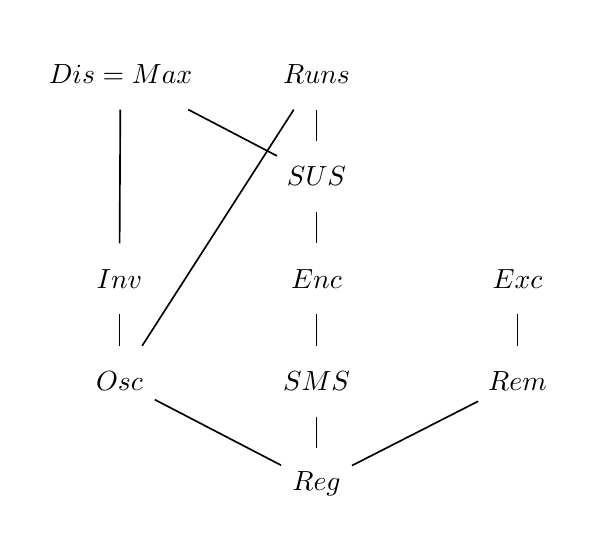
\begin{tikzpicture}[
    		background rectangle/.style={fill=white},
    		show background rectangle,
            auto,
            node distance = 1.3cm,
            semithick
        ]

        \tikzstyle{every state}=[
            draw=none,
            shape=rectangle,
            fill=white
        ]

		\node[state] (reg) {$Reg$};
		\node[state] (sms) [above of=reg] {$SMS$};
		\node[state] (enc) [above of=sms] {$Enc$};
		\node[state] (sus) [above of=enc] {$SUS$};
		\node[state] (runs) [above of=sus] {$Runs$};
		\node[state] (rem) [right=1.5cm of sms] {$Rem$};
		\node[state] (exc) [above of=rem] {$Exc$};
		\node[state] (osc) [left=1.5cm of sms] {$Osc$};
		\node[state] (inv) [above of=osc] {$Inv$};
		\node[state] (dis) [left= 0.9cm of runs] {$Dis=Max$};

        \path[-] (reg) edge node {} (sms);
        \path[-] (sms) edge node {} (enc);
        \path[-] (enc) edge node {} (sus);
        \path[-] (sus) edge node {} (runs);
        \path[-] (reg) edge node {} (rem);
        \path[-] (rem) edge node {} (exc);
        \path[-] (reg) edge node {} (osc);
        \path[-] (osc) edge node {} (inv);
        \path[-] (inv) edge node {} (dis);
        \path[-] (sus) edge node {} (dis);
        \path[-] (osc) edge node {} (runs);
    \end{tikzpicture}
\end{document}
